\section{Thermal Margins and Design Temperatures}

In order to account thermal-model inaccuracies, unpredictable TCS-related events and
any other unexpected events, the following thermal margins have been applied to all
satellite components and the calculated temperatures as defined in [RD02]:
\paragraph{}
\textbf{Thermal Uncertainty Margin}

The Thermal Uncertainty Margin is a margin of safety applied to all calculated
temperatures in order to account for inaccurate physical, environmental and modeling
parameters. A $\pm10 ^\circ C$ uncertainty margin has been taken in this analysis.
\paragraph{}
\textbf{Acceptance Thermal Margin}

The Acceptance Thermal Margin is a contingency to account for unpredictable TCS related
events. A $\pm5 ^\circ C$ acceptance margin for all the components has been considered in
this analysis.

\paragraph{}
\textbf{Qualification Thermal Margin}

The Qualification Thermal Margin is a contingency to account for unexpected events.
A $\pm5 ^\circ C$ qualification margin for all the components has been considered in this analysis.

\begin{figure}[H]
    \centering
    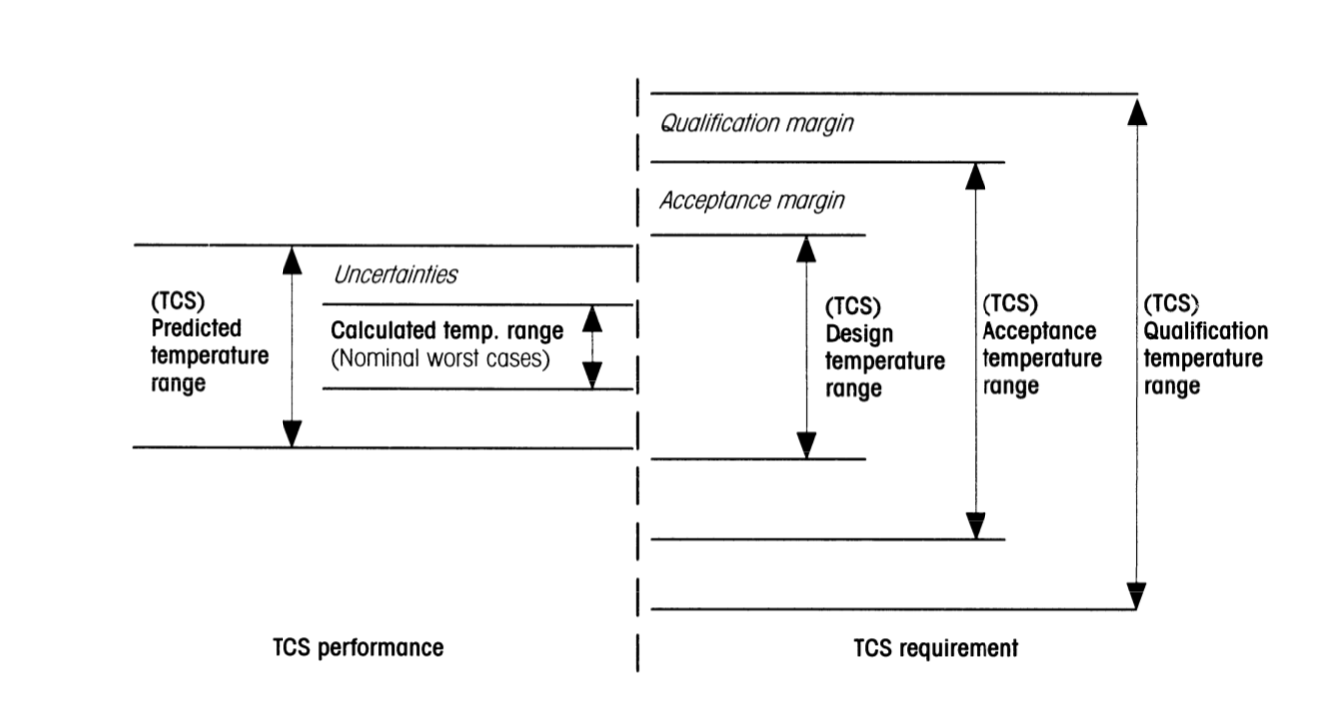
\includegraphics[width=0.6\linewidth]{res/img/2_thermalmargins/DAQTempRangesDiagram.PNG}
    \caption{Temperature Margins Definitions for the TCS}
    \label{fig:DAQTempRanges}
\end{figure}
After the application of the above margins to the Operational Temperature
Ranges (\ref{tab:optemplimits}) as shown in \ref{tab:DAQtemplimits}, the Acceptance and Design Temperature
Ranges are shown in Table \ref{fig:DAQTempRanges}.

\begin{table}[H]
    \centering
    \begin{tabular}{ccccc}
        \toprule
        \multirow{2}{*}{\textbf{Subsystem/Component}} &
        \multicolumn{2}{c}{\textbf{Acceptance Temperature Range (°C)}} &
        \multicolumn{2}{c}{\textbf{Design Temperature Range (°C)}} \\
        \cmidrule(lr){2-3} \cmidrule(lr){4-5}
        & \textbf{Min} & \textbf{Max} & \textbf{Min} & \textbf{Max} \\
        \midrule
        EPS              & -35 & 80  & -30 & 75  \\
        AOCS             & -25 & 80  & -20 & 75  \\
        OBC/COMMS        & -15 & 65  & -10 & 60  \\
        K-Band           & -35 & 80  & -30 & 75  \\
        L-Band           & -35 & 80  & -30 & 75  \\
        Top Board        & -35 & 120 & -30 & 115 \\
        Lateral Boards   & -35 & 120 & -30 & 115 \\
        Bottom Board     & -35 & 80  & -30 & 75  \\
        \midrule
        Battery (Charge)   & 5   & 40  & 10  & 35  \\
        Battery (Discharge) & -15 & 55  & -10 & 50  \\
        \bottomrule
    \end{tabular}
    \caption{Acceptance and design temperature ranges for subsystems and components.}
    \label{tab:DAQtemplimits}
\end{table}
The predicted temperature ranges, i.e. the temperature ranges obtained by analyses (calculated temperature range),
adjusted by the thermal uncertainty margin, must be within the Design Temperature Range under all circumstances.